\documentclass{article}
\usepackage{datatool}
\usepackage{graphicx}
\usepackage[update,prepend,outdir=./]{epstopdf}
\DTLsetseparator{,}

\DTLloaddb{data}{/Users/carlchapman/Documents/SoftwareProjects/tour_de_source/analysis/analysis_output/database.csv}

\begin{document}
Some data from the database:
\\*nObserved: \DTLfetch{data}{key}{nObserved}{value}.
\\*nSkipped: \DTLfetch{data}{key}{nSkipped}{value}.
\\*nAborted: \DTLfetch{data}{key}{nAborted}{value}.
\\*nScanned: \DTLfetch{data}{key}{nScanned}{value}.
\\*nProjectsWithRegex: \DTLfetch{data}{key}{nProjectsWithRegex}{value}.
\\*nPythonFiles: \DTLfetch{data}{key}{nPythonFiles}{value}.
\\*nFilesWithRegex: \DTLfetch{data}{key}{nFilesWithRegex}{value}.

\subsection*{\centerline{REPRESENTING A CORPUS OF REGEXES}}%unnumbered
1. How can we choose a small list of actual regexes to best represent all regexes within a corpus by usage?
\\*a.) What regexes are most frequently used?
\\*b.) What features are most frequently used?
\\*c.) What regexes are most cloned?
\\*d.) What behavioral clustering can be observed?
\\*e.) What syntactic clustering can be observed?
\\*f.) Various synthesis of a-e.


\subsection*{\centerline{CONTEXT AND CORPUS}}%unnumbered

\begin{figure}[!htb]
\centering
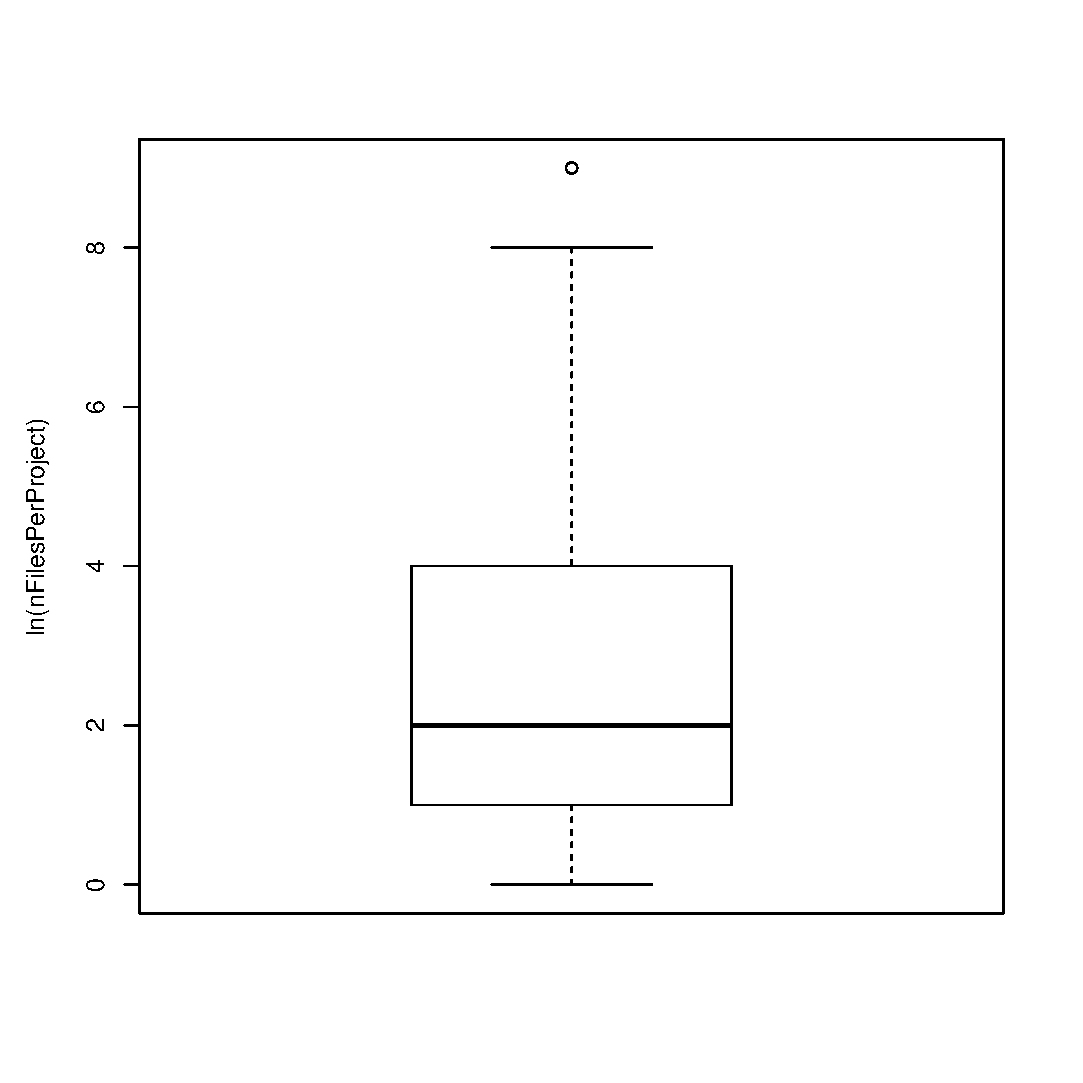
\includegraphics[scale=0.4]{/Users/carlchapman/Documents/SoftwareProjects/tour_de_source/analysis/analysis_output/filesPerProject.eps}
\caption{Example diagram: filesPerProject natural log}
\label{fig:digraph}
\end{figure}

\end{document}
